\documentclass[
LEEC,			% Use this option to select your DEE degree, options: LEEC, LETI
english,		% Select document language, options: portuguese or english
%draft,	% Uncomment for draft mode (no pictures, no links, overfull hboxes) 
%twocolumn
]{DEEclass}

% Use the 'preamble.tex' file (root folder) do add packages and macros. Keep your main.tex file clean.

% FYI, the following packages are preloaded with the document class:
% longtable, xcolor, graphicx, booktabs, caption, csquotes, hyperref,
% calc, listings, datetime2, siunitx, geometry, enumitem

%%%%%%%%%%%%%%%%%%%%%%%%%%%%%%%%%%%%%%%%%%%%%%%%%%%%%%%%%% extra packages
\usepackage{amsmath}		% the main package in the AMS-LATEX distribution
\usepackage{amsfonts}		% extended set of fonts for use in mathematics
\usepackage{amssymb}		% adds new symbols to be used in math mode
\usepackage{mathrsfs}		% math fonts, e.g., Laplace
\usepackage{float}			% provides the H float modifier option
\usepackage{multirow}		% tables \multirow command
\usepackage{subcaption}		% enables subfigures
\usepackage{lscape}			% for landscape mode
\usepackage{verbatim}		% new verbatim environment, 
\usepackage{multicol}		% enables multicolumns 
\usepackage[intoc, english]{nomencl} % add nomenclature
\makenomenclature
\usepackage{etoolbox}       % used for nomenclature, i guess...
\makeglossaries
\usepackage{wrapfig}        % enable wrapping figures graphics
\usepackage{graphicx}       % enable graphics
\let\cleardoublepage=\clearpage     % delete blank pages
%\begin{comment}...\end{comment}, \verbatiminput


%add extra packages if needed here

%%%%%%%%%%%%%%%%%%%%%%%%%%%%%%%%%%%%%%%%%%%%%%%%%%%%%%%%%% temp packages
\usepackage{lipsum}						% for fake text
%\usepackage[textsize=tiny]{todonotes}   % enable To-do notes, use the option "disable" to hide all notes, usage \todo{}

%\usepackage{draftwatermark}			% prints a watermark overlay, uncomment if needed
%\SetWatermarkText{**DRAFT**}
%\SetWatermarkScale{1}
%\SetWatermarkColor[gray]{0.8}

%%%%%%%%%%%%%%%%%%%%%%%%%%%%%%%%%%%%%%%%%%%%%%%%%%%%%%%%%% settings
\AtBeginDocument{					% Rendered PDF metadata:
\hypersetup{pdftitle=\ttitle} 		% Sets the PDF title to your dissertation title
\hypersetup{pdfauthor=\authorname} 	% Sets the PDF author to your name
}

%%%%%%%%%%%%%%%%%%%%%%%%%%%%%%%%%%%%%%%%%%%%%%%%%%%%%%%%%% user defined macros









	
% \makenomenclature

%%%%%%%%%%%%%%%%%%%%%%%%%%%%%%%% REPORT INFORMATION %%%%%%%%%%%%%%%%%%%%%%%%%%%%%%%%%%%%%

\reporttitle{Protocoles Mesures Expérimentales} % Your report title

\author{Kite Design}	% Your name
\studentnumber{0673627662}	% Your student number
\studentemail{1234567@isep.ipp.pt}	% Your student email address  

\advisor{Nome do Orientador}{xxx@isep.ipp.pt}	% Your ISEP advisor name and email
\coadvisor{Nome do Coorientador}{xxx@isep.ipp.pt}	% Your ISEP co-advisor name and email, comment this line if not needed
\company{Nome da Empresa, Lda.}	% The company name where you developed your work, comment this line if not needed
\supervisor{Nome do Orientador da Empresa}{xxx@emailaddress.com} % Your company supervisor name, comment this line if not needed

%%%%%%%%%%%%%%%%%%%%%%%%%%%%%%%%%%%%%%%%%%%%%%%%%%%%%%%%%%%%%%%%%%%%%%%%%%%%%%%%%%%%%%%%%
\begin{document}

\printcoverpage

\tableofcontents

%%%%%%%%%%%%%%%%%%%%%%%%%%%%%%%%%%% MAINMATTER %%%%%%%%%%%%%%%%%%%%%%%%%%%%%%%%%%%%%%%%%

\chapter{Introduction}
\label{ch:Ch0}

Ce bureau d'étude a pour sujet l'équilibre du Kite, sa condition d'existence et sa stabilité. L'objectif final étant de déterminer des paramètres optimaux tels que le towpoint.
\chapter{Travaux précédents (Zoé Marcelet)}
\label{ch:Ch1}

%%%%%%%%%%%%%%%%%%%%%%%%%%%%%%%%%%%% SECTION 1
\section{Modèle Lagragien} 
\label{sec:Ch1.1}

D'après le document \textit{"Dynamics and Control of Single-Line Kites"} de Gonzalo Sanchez-Arriaga (2006),  les formules suivantes permettent d'obtenir l'élévation $\Gamma$ et l'angle d'incidence du vent $\theta$, en fonction du vent et des coefficients aérodynamiques du kite : \\

\begin{figure}[H]
    \centering
    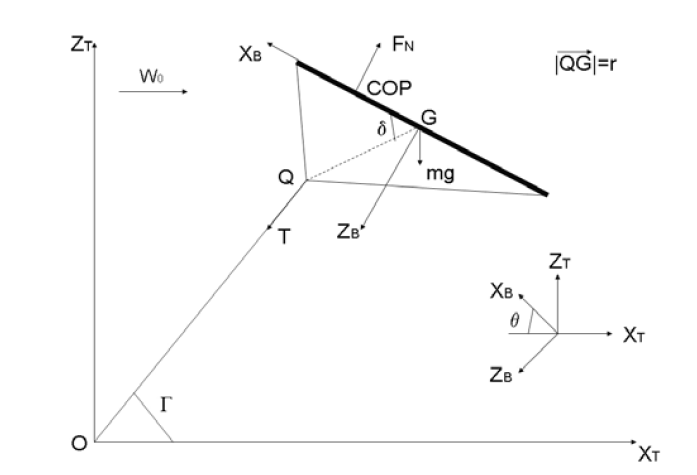
\includegraphics[width=0.5\textwidth]{Pics/01 - Travaux précédents/Picture Sanchez.png}  
    \caption{Schéma du kite au Zénith.}
    \label{fig:sanchez}
\end{figure}

La première équation donne l’angle d’incidence $\theta$ : 
\begin{center}
    \begin{equation}
        cos(\delta - \theta) + \beta (\sigma-cos(\delta))C_N(\theta) = 0
        \label{eq:theta}
    \end{equation}
\end{center}
La deuxieme équation donne l’angle d’élévation $\Gamma$ :
\begin{center}
    \begin{equation}
        \Gamma = tan^{-1}(\frac{\beta C_N (\theta) cos(\theta)-1}{\beta C_N (\theta)sin(\theta)})
        \label{eq:gamma}
    \end{equation}
\end{center}
Avec $\beta = \frac{\rho A W_0^2}{2mg}$ et $\sigma = \frac{X_{cp}}{r}$ \\

Ces équations ont été codées (disponible sur Nextcloud : 06-RESSOURCE/AC-Admin Commun/4-Rapports Stagiaires/Stage Zoé Marcelet/Rapport\_zozo/06\_Topic\_modèle\_aéro\_zenith). \\
\textbf{Elles restent cependant peut concluantes car requièrent les coéfficients aérodynamiques du kite. }
\chapter{Mesure de l'angle d'incidence au Zénith}
\label{ch:Ch2}

%%%%%%%%%%%%%%%%%%%%%%%%%%%%%%%%%%%% SECTION 1
\section{Problème de l'angle de calage $\alpha_0$} 
\label{sec:Ch2.1}

Une première intuition nous amène à penser que la connaissance de l'angle d'élévation et de la géométrie des bridages permet de remonter à l'angle d'incidence $\alpha$

\begin{figure}[H]
    \centering
    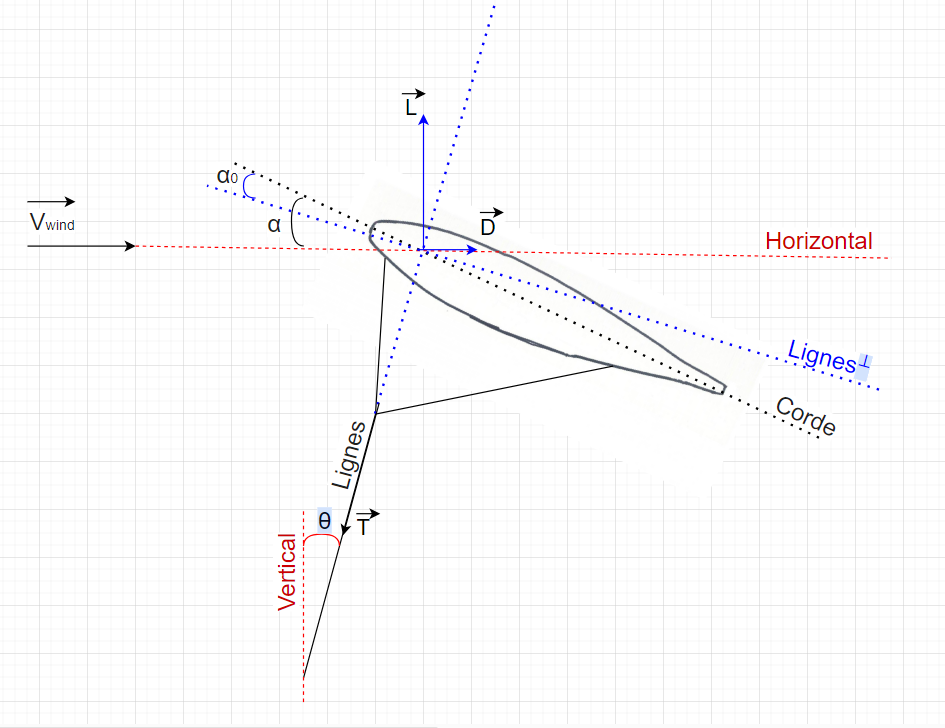
\includegraphics[width=0.5\textwidth]{Pics/02 - Mesure de l'angle d'incidence au Zénith/Schéma Equilibre Zéntih.png}  
    \caption{Schéma des angles qui paramètres le Zénith.}
    \label{fig:Zénith alpha zéro}
\end{figure}

La figure \ref{fig:Zénith alpha zéro}, l'angle $\alpha_0$ dépend de considération aérodynamique, car : 
\begin{center}
    \begin{equation}
        \frac{L}{D} = \frac{1}{tan(\theta)} = \frac{1}{tan(\alpha + \alpha_0)}
    \end{equation}
\end{center}
Ainsi, l'angle que fait le cône de bridage avec les lignes qui le relient au sol s'adapte (via l'angle $\alpha_0$) de sorte à aligner les efforts aérodynamiques avec les lignes des avants. Ainsi, cette angle permet de lier "géométrie" et "aérodynamique" :  

\begin{figure}[H]
    \centering
    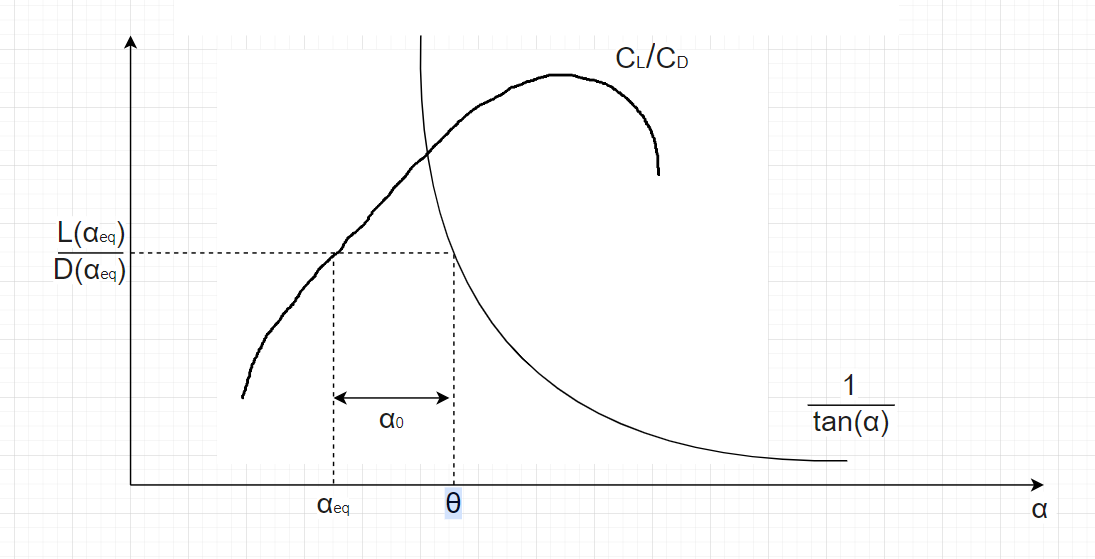
\includegraphics[width=0.5\textwidth]{Pics/02 - Mesure de l'angle d'incidence au Zénith/Schéma Equilibre finesse.png}  
    \caption{Graphique du lien entre finesse (aérodynamique) et l'angle $\alpha_0$}
    \label{fig:Zénith finesse}
\end{figure}

\textbf{Cependant,} la formule à l'équilibre suivante (voir "equilibre kite" pour demo) : 

\begin{center}
    \begin{equation}
        x_T = \frac{L x_F - P x_G -C_{M_0}}{L - P}
    \end{equation}
\end{center}

montre qu'en \textbf{vent fort}, pour $C_{M_0} = 0$, $x_T = x_F$, et donc on peut déterminer géométriquement $\alpha_0$ ! \textbf{Donc la mesure de l'angle $\theta$ permet de remonter à $\alpha$ et à la finesse $\frac{L}{D}$}\\

%%%%%%%%%%%%%%%%%%%%%%%%%%%%%%%%%%%% SECTION 2
\section{Utiliser un capteur de tension pour les A et les B au niveau du kite} 
\label{sec:Ch2.2}

L'idée est que notre système \{kite+bridages\} se comporte comme un pendule inversé. Mesurer les tensions dans les A et les B permet de mesurer la position de la résultante aérodynamique le long du kite et ainsi de prédire son angle d'incidence $\alpha$ en s'affranchissant de la polaire aérodynamique du kite. 

\begin{figure}[H]
    \centering
    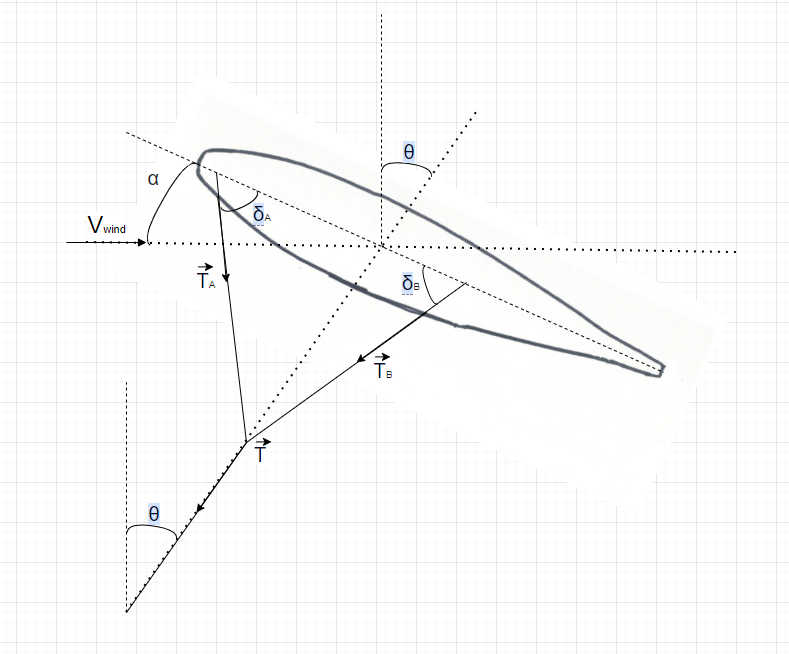
\includegraphics[width=0.5\textwidth]{Pics/02 - Mesure de l'angle d'incidence au Zénith/Schéma Equilibre capteurs tension AB.png}  
    \caption{Schéma des tensions dans les bridages}
    \label{fig:Zénith tensions AB}
\end{figure}

Le graphe \ref{fig:Zénith tensions AB} permet d'écrire la relation suivante : 
\begin{center}
    \begin{equation}
        T_A cos(\delta_A) - T_B cos(\delta_B) = T cos(\frac{\pi}{2} +\alpha - \theta)
    \end{equation}
\end{center}

et ainsi d'en déduire :

\begin{center}
    \begin{equation}
        \alpha = \theta + sin^{-1}(\frac{T_B cos(\delta_B) - T_A cos(\delta_A)}{T}))
        \label{eq:alpha}
    \end{equation}
\end{center}

Ainsi, on peut déterminer l'angle d'incidence $\alpha$ à partir de :
\begin{itemize}
    \item T : la tension des avants ( capteur "3 axes" )
    \item $\theta$ : $\frac{\pi}{2}$ - l'angle d'élévation (capteur "IMU")
    \item $T_A$ : la tension dans les A au point d'attache du kite (capteur "cyclops")
    \item $T_B$ : la tension dans les B au point d'attache du kite (capteur "cyclops")
    \item $\delta_A$ : l'angle des A par rapport à la corde moyenne du kite (surfplan ou au laser)
    \item $\delta_B$ : l'angle des B par rapport à la corde moyenne du kite (surfplan ou au laser)
\end{itemize}

%%%%%%%%%%%%%%%%%%%%%%%%%%%%%%%%%%%% SECTION 3
\section{La sonde pitot} 
\label{sec:Ch2.3}

L'équilibre au Zéntih permet d'obtenir : 

\begin{equation}
    \begin{cases}
        L = P + T sin(\theta) \\
        D = T cos(\theta) \\
        0 = C_{M_0} + (x_T - x_F) (L cos(\alpha) + D sin(\alpha)) - P cos(\alpha) (x_T - x_G)
    \end{cases}
    \label{eq:equilibre aero}
\end{equation}


Ainsi, couplé avec les résultats de la section \ref{sec:Ch2.2}, on peut mesure $L(\alpha), D(\alpha)$ et $\alpha$ à partir des capteurs cités dans ce même chapitre. 
Cependant, la connaissance du vent en altitude, à 50m de haut, est incertaine et l'ajout de la sonde pitot, fixée à un kite stable, permet d'obtenir avec précision les coéfficients $SC_L$ et $SC_D$ via :

\begin{equation}
    \begin{cases}
        L = \frac{1}{2} \rho V^2 SC_L \\
        D = \frac{1}{2} \rho V^2 SC_D 
    \end{cases}
    \label{eq:clcd}
\end{equation}

Les modèles de couches limites sont de la forme 
\begin{equation}
        u(z) = -C \mu e^{\frac{z}{\lambda}} sin(\frac{z}{\lambda}) \\
\end{equation}

où les différents coéfficients sont charactéristiques du lieu. (\textbf{Source :} \textit{Sébastien Blein. Observation et modélisation de couche limite atmosphérique stable en relief complexe : le processus turbulent d’écoulement catabatique. Météorologie. Université Grenoble Alpes, 2016. Français. ffNNT : 2016GREAI023ff. fftel-01622676f} - équation 2.69 du chapitre 2.3.1 (modèle de Prandtl)). \\

Un autre modèle est celui proposé par Fechner et Schmehl dans "Model-Based Efficiency Analysis ofWind Power Conversion by a Pumping Kite Power System" :  
\begin{equation}
    v_w = v_{w,g} (\frac{\overline{h}}{ 10 m })^{\alpha} \\
\end{equation}

Avec $v_{w,g}$ la ground wind speed à 10 m, $\overline{h}$ la hauteur moyenne du kite, et $\alpha$ un coefficient dont la valeurs standard est 1/7, là où en offshore $\alpha$ vaut plutôt 0.11\\

Aussi, la connaissance de $\rho$ est nécessaire. La formule suivante peut être utilisée :
\begin{equation}
    \rho = \rho_{0} e^{-\frac{\overline{h}}{H_{\rho}}} \\
\end{equation}
avec $H_{\rho} = 8:55 km$ et $\rho_{0} = 1.225 Kg.m^{-3}$

\textbf{Ainsi, on propose de mesurer les vitesses à différentes hauteurs grâce à la sonde pitot afin d'établir un modèle de couche limite pour un lieu (\textit{plage de Pereire}) et une provenance de vent (\textit{Nord-Ouest-Sud}) [l'état. de la couche limite dépend des obstacles qui précèdent le lieu de mesure]}

%%%%%%%%%%%%%%%%%%%%%%%%%%%%%%%%%%%% SECTION 4
\section{Conclusion} 
\label{sec:Ch2.4}

Muni des capteurs
\begin{itemize}
    \item 3 axes
    \item IMU
    \item Cyclops
    \item Sonde pitot\\
\end{itemize} 

On propose de :
\begin{itemize}
    \item Mesurer $\alpha$ grace à l'équation \ref{eq:alpha}, et le couple $(L(\alpha);D(\alpha))$ grace à l'équation \ref{eq:equilibre aero}. Répéter l'essai pour différentes valeurs de \textbf{TowPoint}
    \item Déterminer un modèle de couche limite grâce à la sonde pitot en mesurant des valeurs de vitesse vent à différentes hauteurs (\textit{réunion avec Delft mercredi 16/10 et voir avec mecatro pour filtrer/moyenner mesures})
    \item Déduire grâce à \ref{eq:clcd} les coéfficients aéro au zénith.
\end{itemize} 
\chapter{Mesure de l'angle d'incidence au Zénith}
\label{ch:Ch3}

%%%%%%%%%%%%%%%%%%%%%%%%%%%%%%%%%%%% SECTION 1
\section{Calcul de la finesse en pleine fenêtre} 
\label{sec:Ch3.1}

\textbf{En l'absence d'angle de calage} ($\alpha_0 = 90$\textdegree), on a l'équilibre dynamique qui devient :
\begin{center}
    \begin{equation}
        L sin(\theta) - D cos(\theta) = t sin(\alpha_0) \Rightarrow \frac{D}{L} = tan(\alpha)
        \label{eq : l_over_d}
    \end{equation}
\end{center}

ainsi, Fechner et Schmehl dans "Model-Based Efficiency Analysis ofWind Power Conversion by a Pumping Kite Power System" proposent : 

\begin{center}
    \begin{equation}
        v_a^2 = (v_w cos(\beta) cos(\Phi) - v_{t,0})^2( 1 + (\frac{L}{D})^2)
    \end{equation}
\end{center}

par relation de pythagore, avec ici $\beta$ est l'angle d'élévation, $\Phi$ l'angle azimuth, et $v_{t,0}$ la reel\_out speed utilisée par kite-power (nul dans notre cas d'un point fixe)\\

Finalement on obtient la relation : 
\begin{center}
    \begin{equation}
        v_a = ( cos(\beta) cos(\Phi) - \frac{v_{t,0}}{v_w}) v_w \sqrt{ 1 + (\frac{L}{D})^2}
    \end{equation}
\end{center}

\textbf{Cette relation permet d'obtenir la finesse du kite, en shoot (vitesse max) en focntion de l'élévation, du vent réel, et du vent relatif !}

\section{Influence des lignes}

Quand on parle de finesse, on parle en rélalité de la \textbf{finesse de l'ensemble du système Kite + Ligne}, soit $finesse = \frac{C_L^k}{C_D^k + C_D^{lignes}}$\\

Fechner et Schmehl dans "Model-Based Efficiency Analysis ofWind Power Conversion by a Pumping Kite Power System" proposent pour prendre en compte la trainée des lignes supérieures uniquement, la portion des lignes qui se déplace à la vitesse du kite, la portion inférieur étant alors considérée fixe :

\begin{equation}
    C_{D, eff}^{lignes} \approx  0.31 \overline{l} \frac{d}{A_{kite}} C_D^{lignes}
\end{equation}

Dès lors on a $C_D = C_D^k + C_{D, eff}^{lignes} $ et \textbf{en l'absence d'angle de calage}:

\begin{equation}
    F_{t, max} = \frac{1}{2} \rho v_a^2 A_{kite} C_D \sqrt{1 + (\frac{L}{D})^2}
\end{equation}


%%%%%%%%%%%%%%%%%%%%%%%%%%%%%%%%%%%%%%%%%%%%%%%%%%%%%%%%%%%%%%%%%%%%%%%%%%%%%%%%%%%%%%%%% BIBLIOGRAPHY


\end{document}